\documentclass{beamer}
\usepackage{subfig}


\title{Introduction to Machine Learning}
\author{Prof. Alessandro Lucantonio}
\institute{Aarhus University - Department of Mechanical and Production Engineering}
\date{?/?/2023}

\begin{document}
	
	\frame{\titlepage}
	
	\begin{frame}
		\frametitle{What is Machine Learning?}
		\begin{itemize}
			\item Arthur Samuel (1959). Machine learning is a “Field of study that gives computers the ability to learn without being explicitly programmed”.
			\item Tom Mitchell (1998). “A computer program is said to learn from experience E with respect to some class of tasks T and performance measure P, if its performance at tasks in T, as measured by P, improves with experience E”.
		\end{itemize}
		
	\end{frame}

	\begin{frame}		
		\frametitle{Some applications - Image recognition}
		\begin{figure}
			\centering
			\subfloat[\centering]{{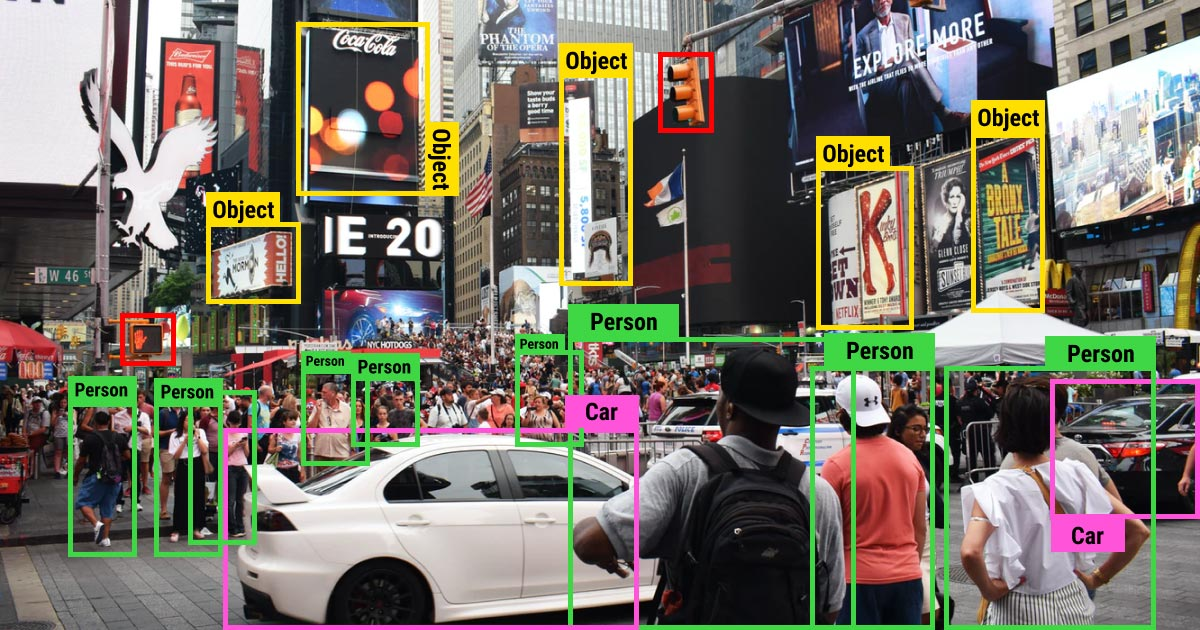
\includegraphics[scale=0.13]{images/image-recognition-1}}}
			\qquad
			\subfloat[\centering]{{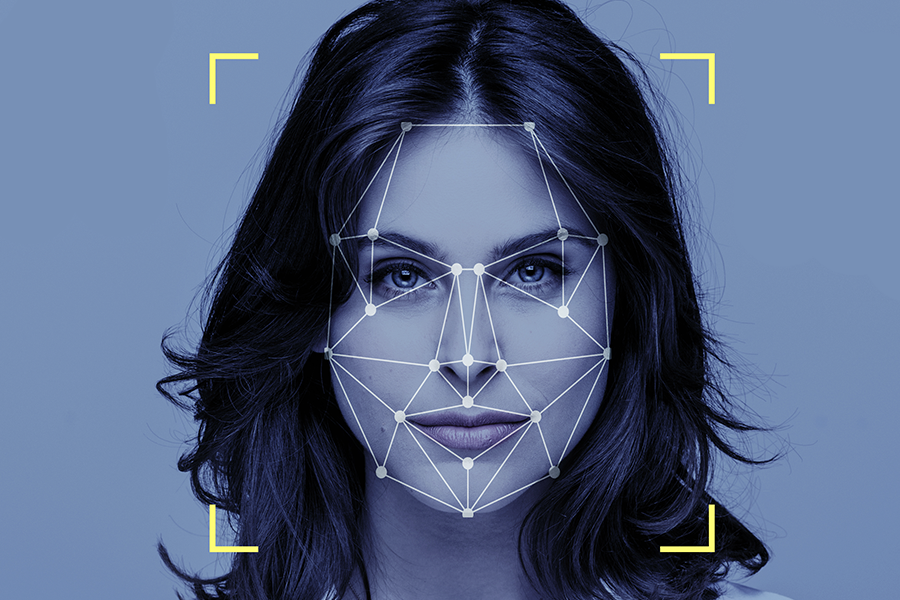
\includegraphics[scale=0.13]{images/image-recognition-2}}}
		\end{figure}
	Two examples of image recognition. 
	
	(a) Labelling different entities in a given image. 
	
	(b) Face recognition (as in our smartphones).
	\end{frame}

	\begin{frame}
		\frametitle{Some applications - Speech and voice recognition}
		\begin{figure}
			\centering
			\subfloat[\centering]{{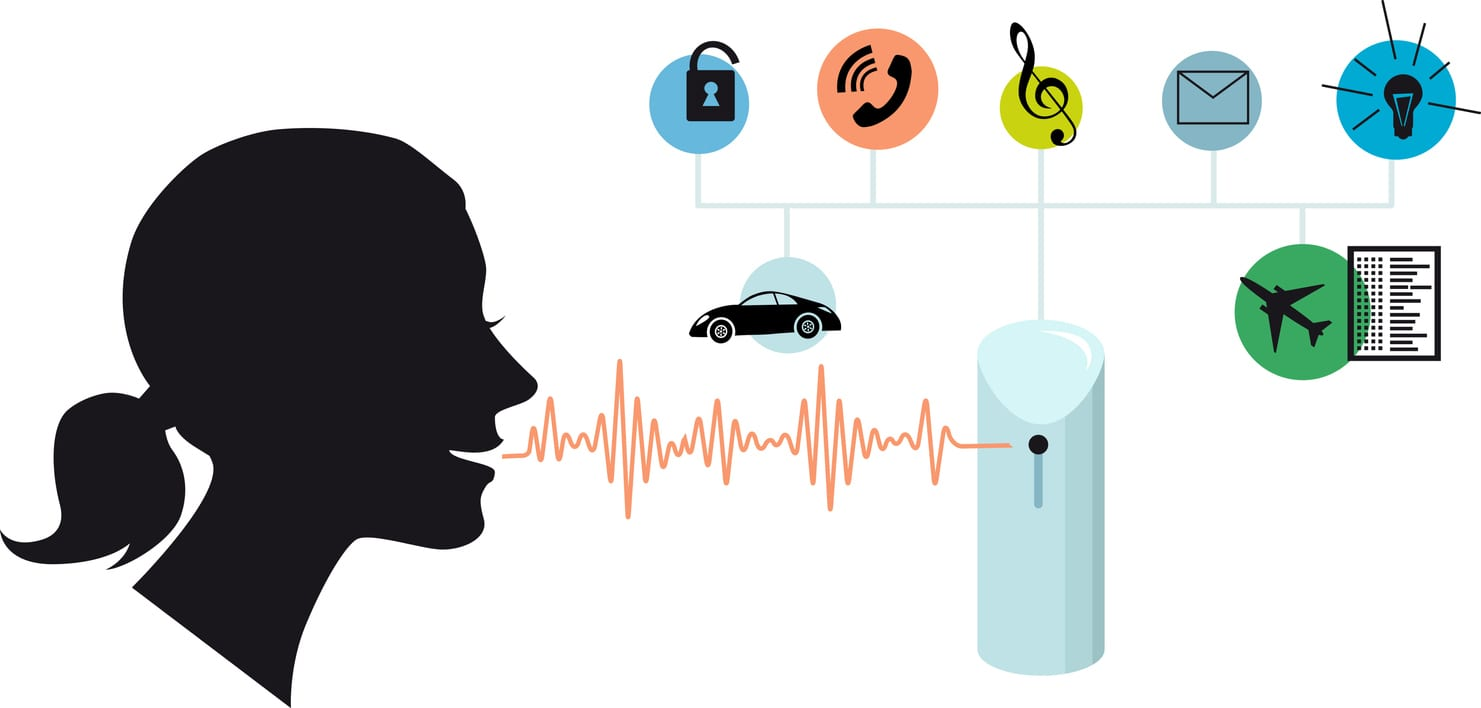
\includegraphics[scale=0.13]{images/speech-recognition-1}}}
			\qquad
			\subfloat[\centering]{{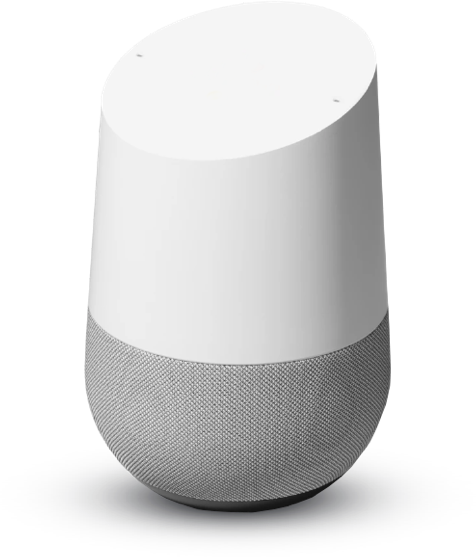
\includegraphics[scale=0.13]{images/speech-recognition-2}}}
		\end{figure}
	Two examples of speech and voice recognition. 
	
	(c) A general idea of speech recognition. 
	
	(d) Apple Siri.
	
	\end{frame}

	\begin{frame}
		\frametitle{Some applications - Self driving cars}
		\begin{figure}
			\centering
			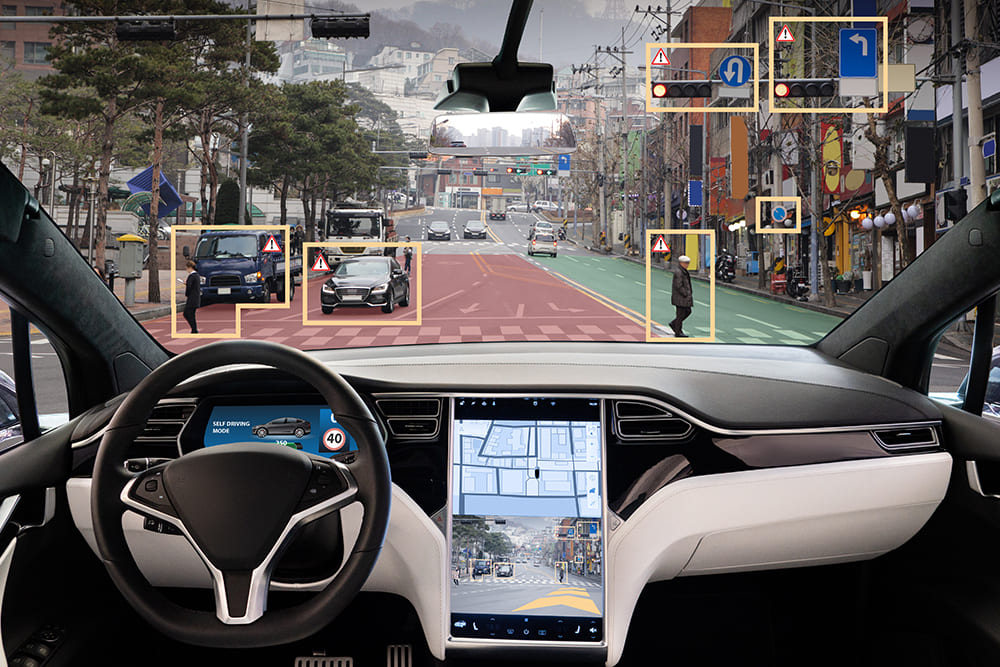
\includegraphics[scale=0.3]{images/self-driving-1}
		\end{figure}
		Using e.g. image recognition, companies are building self-driving cars increasingly efficient.
		
	\end{frame}

	\begin{frame}
		\frametitle{Some applications - Email spam filtering}
		\begin{figure}
			\centering
			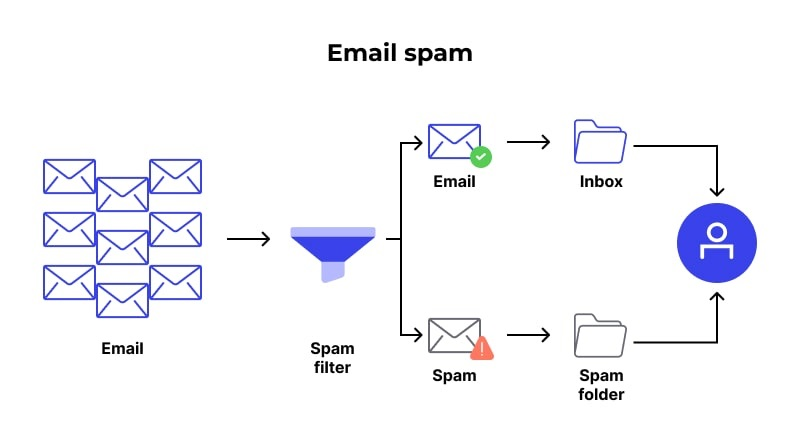
\includegraphics[scale=0.5]{images/spam-filtering-1}
		\end{figure}
		Determine if a given email is spam or not.
		
	\end{frame}

	\begin{frame}
		\frametitle{Some applications - Learning how to play games}
		\begin{figure}
			\centering
			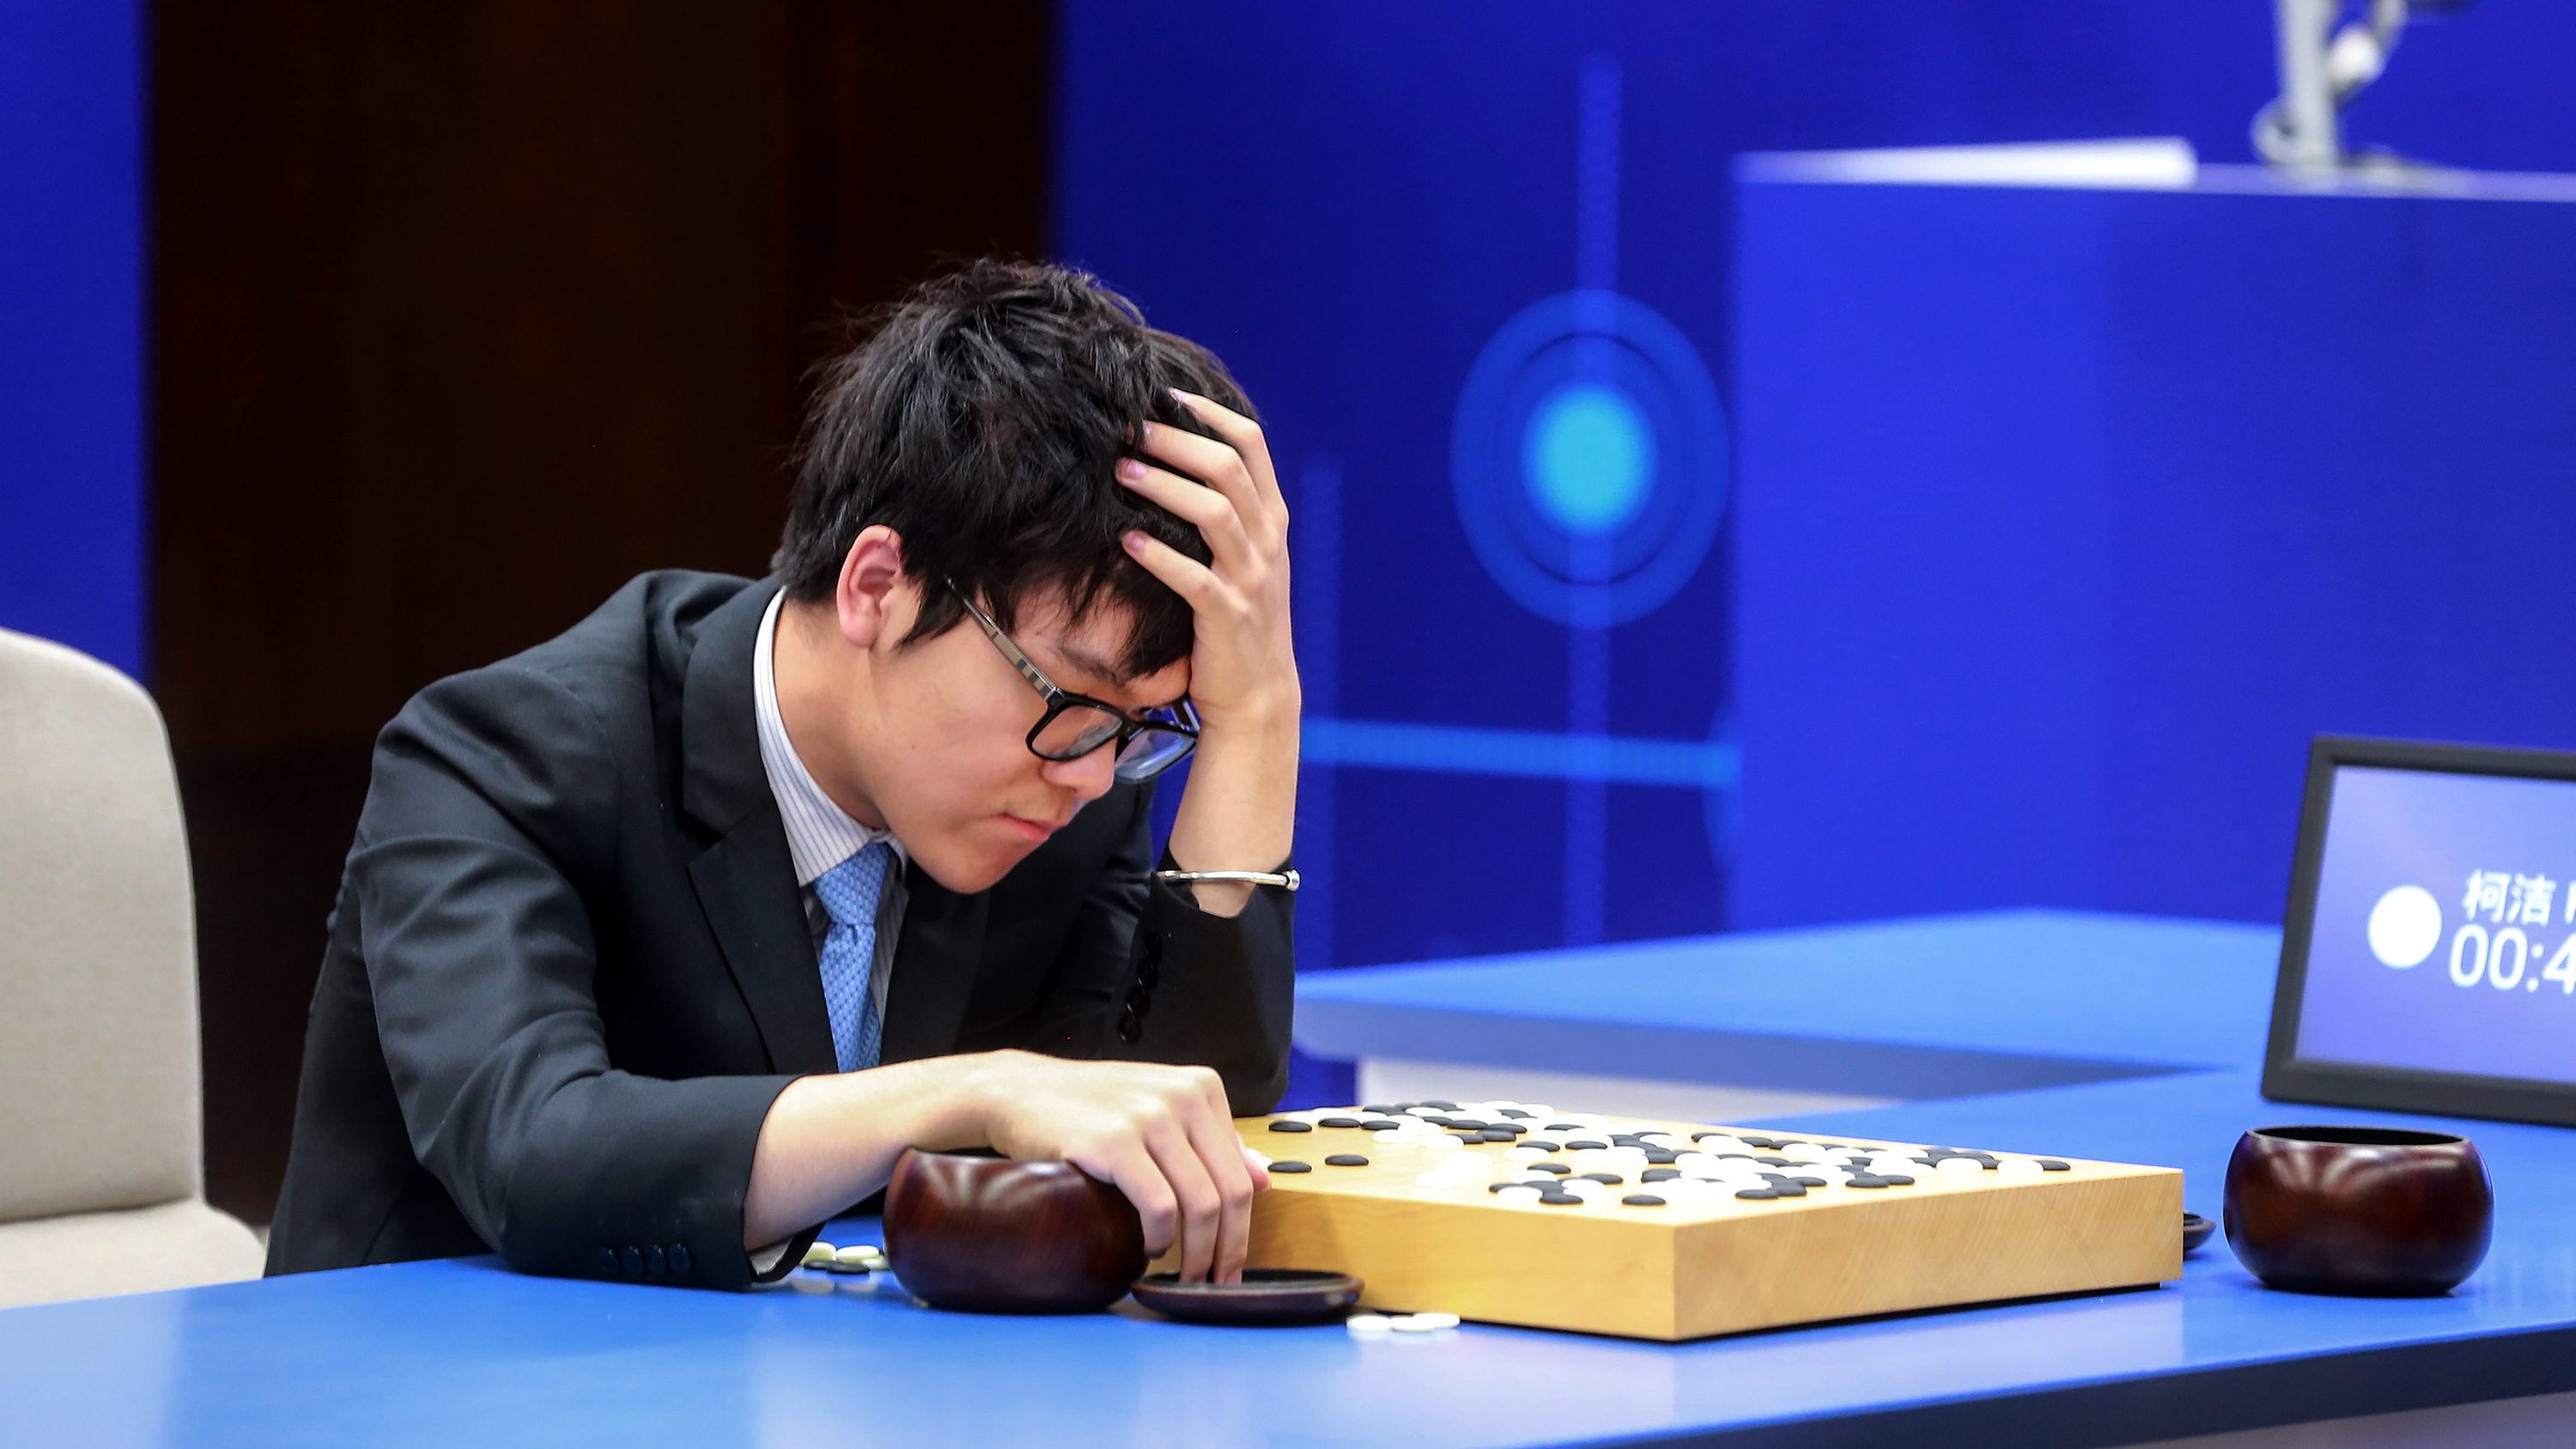
\includegraphics[scale=0.3]{images/alphago}
		\end{figure}
	
	"AlphaGo is the first computer program to defeat a professional human Go player, the first to defeat a Go world champion, and is arguably the strongest Go player in history." 
	
	More info: \href{https://www.deepmind.com/research/highlighted-research/alphago}{https://www.deepmind.com/research/highlighted-research/alphago}
		
		
	\end{frame}

	\begin{frame}
		\frametitle{Supervised Learning}
		In \textbf{supervised learning}, a dataset of input-output relations is provided.
		The learning is supervised because we already know how the current looks like.
		
		Two type of supervised learning problems:
		\begin{itemize}
			\item \textbf{Regression}. Predict results within a continuous output.
			
			Example: Predict the price of an house given its size.
			\item \textbf{Classification}.  Predict results within a discrete output (categorical data).
			
			Example: Given an email, predict if it is spam or not (\textsl{binary classification})
		\end{itemize}
	\end{frame}

	\begin{frame}
		\frametitle{Unsupervised Learning}
		In \textbf{unsupervised learning}, we have no idea how the output looks like (unlabeled data). We have to derive structure and different relationships from data.
		
		Examples:
		\begin{itemize}
			\item Take a collection of essays and find a way to automatically group them based on word frequency, sequence length, page counts etc.
			\item Recommender systems. Automatically provide suggestions for an item
			that is most pertinent to a particular user.
		\end{itemize} 
		
	\end{frame}
	
\end{document}